\section{Week 5}
%\begin{itemize}
    
    %\item Draw a figure of the organization of the system.
    %\item Relate the organization of the system to the different types of operation systems discussed in the text book by Tanenbaum and Bos.
    %\item What kind of operating system is it? Why?
    %\item How is the system booted? Outline each step.
    
%\end{itemize}

\subsection{The system skeleton}

The system as given in the skeleton is composed of some start up files such as \texttt{entry.s}, defining the environment and certain low level protocols. This involves, disabling interrupts, clearing any statically allocated variables, setting up the kernel stack, and further down the line, call \texttt{kernel\_init} found in \texttt{kernel.c}. The \texttt{startup\_32.s} file contains the protocol for starting a program, setting up the needed environment, and calling the respective main function. The kernel implementation is seen in the \texttt{kernel} and \texttt{kernel\_customization} files, together with the \texttt{video.c} file defining how information is displayed on the monitor. In the labs, we are mainly concerned with the development of the file \texttt{video.c} together with the \texttt{kernel\_customization} header and \texttt{c} file. 

\begin{figure}[H]
    \centering
    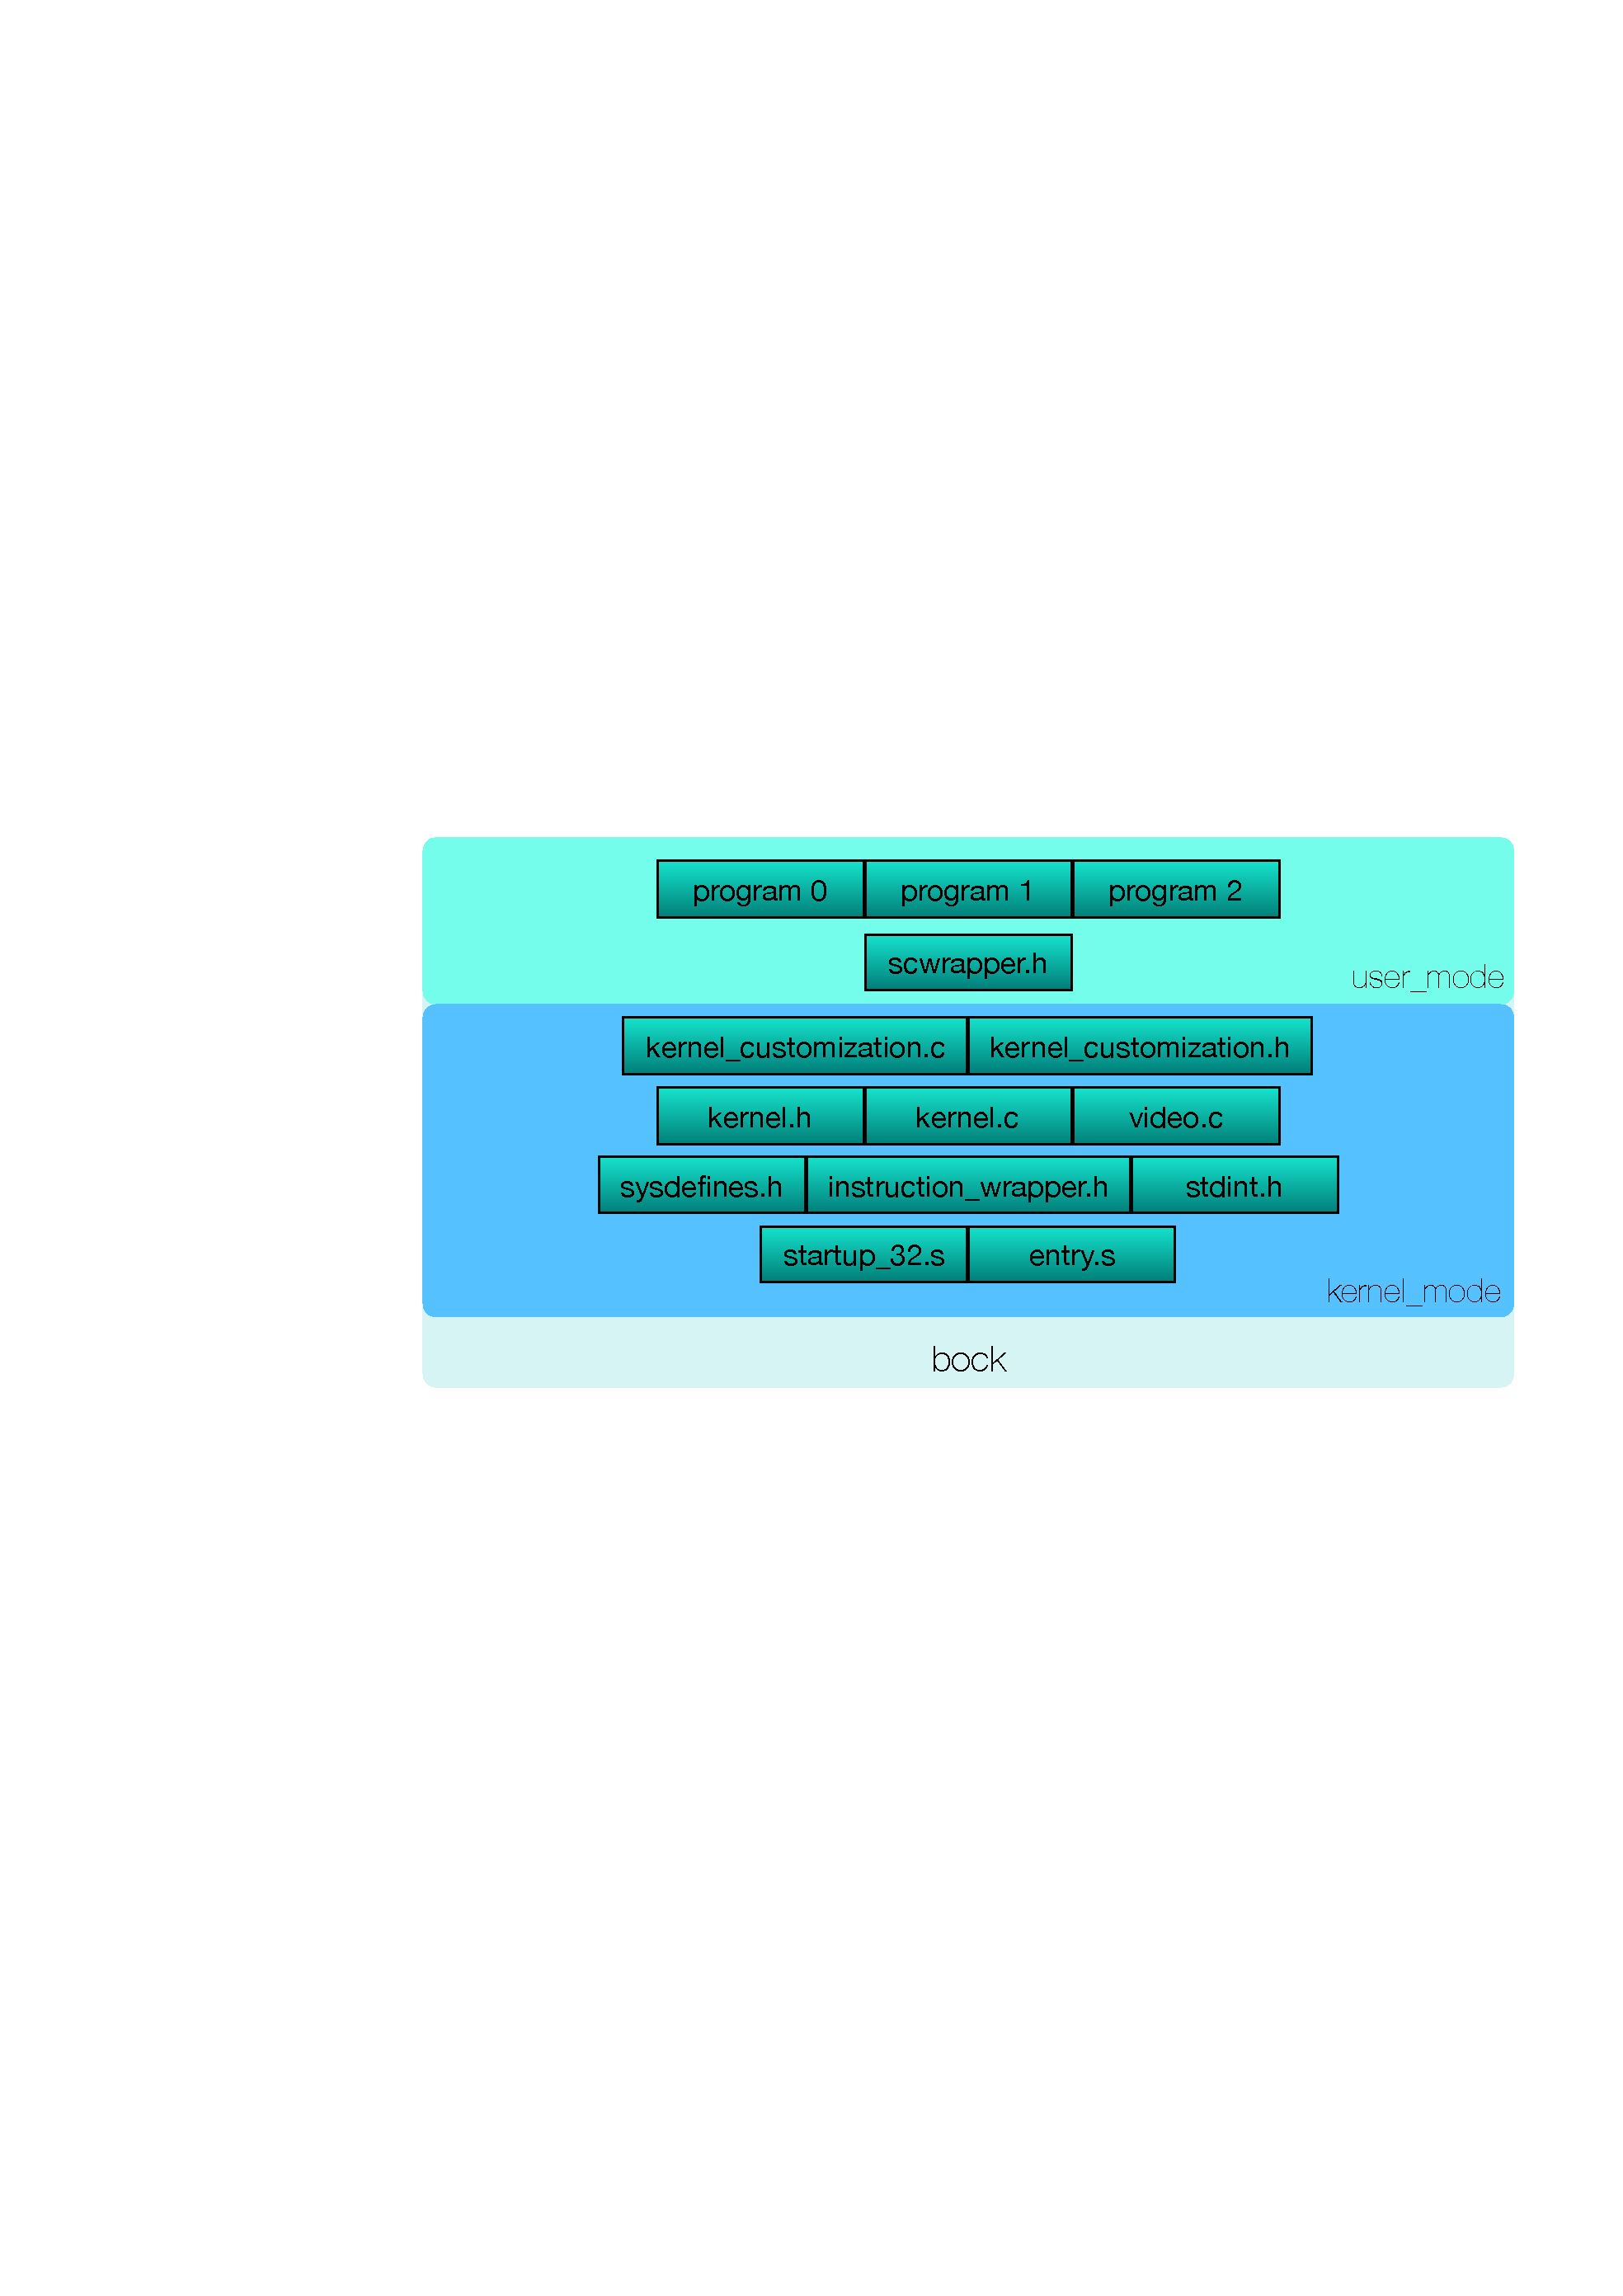
\includegraphics[width=\linewidth]{fig/system_organization.pdf}
    \caption{Organization of the system implementation.}
    \label{fig:sys_org}
\end{figure}

The programs run in \texttt{user\_mode}, and in order to call system calls executed in \texttt{kernel\_mode}, the \texttt{scwrapper.h} acts as a trap, switching to \texttt{kernel\_mode} using the assembly call \texttt{sysenter} and passing the appropriate parameters on the current threads registers. The \texttt{sysenter} entry point protocol is executed in \texttt{entry.s} which calls the \texttt{handle\_system\_call} function implemented in the file \texttt{kernel\_customization.c}. Once the system call has executed, the system returns to \texttt{user\_mode}, and the program continues. 


Other files like \texttt{instruction\_wrappers.h}, \texttt{sysint.h} and \texttt{sysdefines.h} contain macros, type definitions and assembly instruction wrappers accessible to the kernel. The layering of these implementations are outlined in figure \ref{fig:sys_org}.

Since the different system calls and kernel operations are implemented inside the kernel, this is not a micro-kernel operating system. All resource management is handled through system calls, and not directly, meaning this is not an exo-kernel operating system, which means, that we in fact have a monolithic operating system. For a monolithic operating system, all kernel operations are accessible within \texttt{kernel\_mode}, which is also what we experience in our system. 

In figure \ref{fig:sys_org} we have \texttt{boch} at the very bottom, since this is the program simulating our system in which we launch the operating system. Boch itself is close enough to the actual hardware that the operating system may have access directly to hardware, meaning that the bottom layer could be replaced with hardware.
